\documentclass[11pt]{article}
\usepackage{myz310e-notes}
\hypersetup{pdftitle={Neighbourhood methods: nearest neighbours, Parzen windows and distances},pdfauthor={Emre Onur Kahya},pdfsubject={MYZ 310E Machine Learning in Physics, Fall 2026, lecture note 5 (week 3)}}

\begin{document}
\NoteTitle{5}{3}{Neighbourhood methods: nearest\\ neighbours, Parzen windows and distances}{Neighbourhood methods}{%
Neighbourhood methods predict at a point by letting nearby training examples vote. They need no training, make no
assumption about the shape of the target function, and handle classification, regression and density estimation
with one formula. This note develops $k$-nearest neighbours and Parzen windows (kernel smoothing and kernel density
estimation), discusses the distances they rely on, and shows that the same ideas power retrieval in today's AI
systems and the attention mechanism of transformers. Model selection follows Note~4; the geometry of high dimension
follows Note~3.}

\section{Let the neighbours vote}\label{sec:knn}

Fix a distance $d(\cdot,\cdot)$ on the input space, Euclidean unless stated otherwise. For a query $\x$, let
$N_k(\x)$ be the set of indices of the $k$ training points closest to $\x$. The \emph{$k$-nearest-neighbour} ($k$-NN)
prediction averages their targets. All three tasks fit one formula,
\begin{equation}\label{eq:weighted}
  \bar{\vect{y}}(\x) = \frac{\sum_{i=1}^n w_i(\x)\, \vect{t}_i}{\sum_{i=1}^n w_i(\x)}, \qquad
  w_i(\x) = \ind{i \in N_k(\x)},
\end{equation}
with a task-dependent target encoding $\vect{t}_i$ and read-out:
\begin{itemize}
\item \textbf{regression}: $\vect{t}_i = y_i$ and $f(\x) = \bar{\vect{y}}(\x)$, the mean target of the neighbours;
\item \textbf{classification with $m$ classes}: $\vect{t}_i = \mathrm{onehot}(y_i) \in \{0,1\}^m$, so
$\bar{\vect{y}}(\x)$ is the vector of class frequencies among the neighbours --- an estimate of $P(Y = \cdot \mid
\X = \x)$ --- and $f(\x) = \argmax_c \bar y_c(\x)$, the majority vote;
\item \textbf{binary classification} with $y_i \in \{-1, +1\}$: $f(\x) = \operatorname{sign} \bar y(\x)$.
\end{itemize}
Like the histograms of Note~3, $k$-NN replaces $\E[Y \mid \X = \x]$ by an average over a neighbourhood, but the
neighbourhood is now centred on the query and adapts its size to the local density of data: small where examples are
plentiful, large where they are sparse. No cell is ever empty.

Neighbourhood methods are called \emph{non-parametric}: they assume nothing about the form of $f$, and their
``parameters'' are the training set itself, which must be stored. Their hyperparameters --- $k$ and the distance ---
are chosen on validation data as in Note~4.

\paragraph{Decision regions} For $k = 1$, each training point owns the region of space closer to it than to any
other point, its \emph{Voronoi cell}. The classifier predicts the label of the cell's owner, so the decision boundary
is made of pieces of perpendicular bisectors between differently labelled neighbours (Figure~\ref{fig:voronoi}). It
can be arbitrarily complex: one mislabelled point carves out its own island.

\begin{figure}[h]
\centering
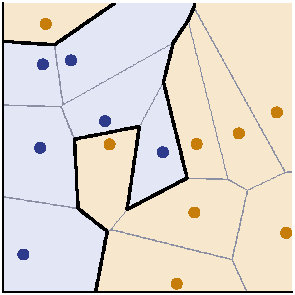
\includegraphics[width=0.36\linewidth]{figures/voronoi.pdf}
\caption{The 1-NN classifier for 14 points. Thin lines: Voronoi cells; thick line: decision boundary; shading:
predicted class.}
\label{fig:voronoi}
\end{figure}

\paragraph{The choice of $k$} Figure~\ref{fig:knnk} shows $k$-NN on 300 points from two interleaved half-moons.
With $k = 1$ the training error is zero and the boundary follows every noisy point; the test error is 9.2\%. With
$k = 15$ the boundary is smooth and training and test errors agree at about 6\%. With $k = 151$, half the training set
votes everywhere, the boundary is too simple to follow the moons and both errors rise to about 19\%. Small $k$ means
low bias and high variance; large $k$ the reverse (Note~4, Section~6). In the limit $k = n$ every query receives the
overall majority class.

\begin{figure}[h]
\centering
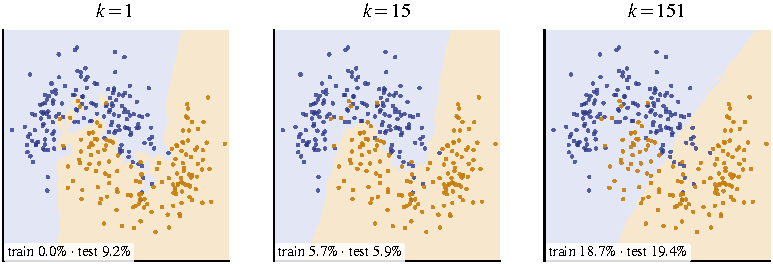
\includegraphics[width=\linewidth]{figures/knn_k.pdf}
\caption{$k$-NN classification of 300 training points; errors on the training set and on 3000 test points.}
\label{fig:knnk}
\end{figure}

\paragraph{What theory guarantees} With enough data, nearest neighbours are close to the query and the method
approaches the ideal. As $n \to \infty$, the error of $1$-NN is at most twice the Bayes error (for two classes,
$R^* \le R_{1\text{-NN}} \le 2R^*(1 - R^*)$)~\cite{cover1967}, and $k$-NN is \emph{consistent} --- its risk converges to
the Bayes risk for every distribution --- if $k \to \infty$ while $k/n \to 0$~\cite{stone1977}. The catch is the rate:
in $d$ dimensions the distance to the nearest neighbour shrinks only like $n^{-1/d}$, and Note~3 showed what that
means for $d = 100$.

\section{Computing neighbours}\label{sec:compute}

The algorithm is short. Training stores $X \in \R^{n \times d}$ and the targets. Prediction for a batch of queries
computes all squared distances with the matrix identity of Note~1, Section~6, selects the $k$ smallest per row and
averages:

\begin{verbatim}
def knn_classify(Xtr, ytr, Xq, k, m):        # ytr: integer labels 0..m-1
    D = sq_distances(Xq, Xtr)                 # (q, n), Note 1
    idx = np.argpartition(D, k - 1, axis=1)[:, :k]   # k nearest, unordered
    votes = np.eye(m)[ytr[idx]].sum(axis=1)   # (q, m) class counts
    return votes.argmax(axis=1)
\end{verbatim}

Partial selection (\texttt{argpartition}) finds the $k$ smallest of $n$ numbers in $O(n)$ time; a full sort would
cost $O(n \log n)$.

\begin{center}\small
\begin{tabular}{@{}lll@{}}
\toprule
 & Brute force & Approximate index (e.g.\ graph-based) \\
\midrule
Memory & $O(nd)$ & $O(nd)$ plus the index \\
Training & none (store the data) & build the index, roughly $O(n \log n)$ distance evaluations \\
Prediction per query & $O(nd)$ & roughly $O(d \log n)$, returns \emph{most} true neighbours \\
\bottomrule
\end{tabular}
\end{center}

Training is free and prediction is expensive --- the opposite of most models. Exact tree structures such as $k$-d
trees prune the search in low dimension but degrade to brute force as $d$ grows, another face of the curse. Large
systems therefore accept \emph{approximate} neighbours: graph-based indices such as HNSW~\cite{malkov2020} and
compressed vector codes on GPUs~\cite{johnson2021} make collections of billions of vectors searchable, at the price
of occasionally missing a true neighbour.

\begin{modern}{nearest neighbours inside AI systems}
Nearest-neighbour search in embedding space (Note~1, Section~3) is everywhere. \emph{Retrieval-augmented generation}
embeds a question, retrieves the nearest passages from a document collection and gives them to a language model as
context~\cite{lewis2020}; the ``vector databases'' behind such systems are approximate $k$-NN indices. A language
model can also be improved without retraining by interpolating its next-token distribution with a $k$-NN estimate
computed from a datastore of contexts~\cite{khandelwal2020} --- exactly the classification rule \eqref{eq:weighted}
with tokens as classes. And self-supervised vision models are routinely evaluated by the accuracy of a $k$-NN
classifier on their features: if a simple vote among neighbours works, the representation has organised the data
well.
\end{modern}

\section{Parzen windows: soft neighbourhoods}\label{sec:parzen}

\paragraph{Hard windows} Instead of the $k$ nearest points, let every point within a fixed radius $h$ vote:
$w_i(\x) = \ind{d(\x_i, \x) < h}$ in \eqref{eq:weighted}. The neighbourhood now has fixed size and variable
population; in sparse regions it may be empty, and a default prediction is needed, as for histograms.

\paragraph{Soft windows} Better still, let \emph{all} training points vote with weights that decrease smoothly with
distance, $w_i(\x) = K(\x_i, \x)$ for a \emph{kernel} $K$. The most common choice is the Gaussian (radial basis
function) kernel
\[
  K_\sigma(\x_i, \x) = \exp\!\left( -\frac{\norm{\x - \x_i}^2}{2\sigma^2} \right),
\]
whose normalising constant cancels in the ratio \eqref{eq:weighted}. Regression with these weights,
\begin{equation}\label{eq:nw}
  f(\x) = \frac{\sum_i K_\sigma(\x_i, \x)\, y_i}{\sum_i K_\sigma(\x_i, \x)},
\end{equation}
is the Nadaraya--Watson estimator; classification uses one-hot targets and an $\argmax$, exactly as for $k$-NN. The
width $\sigma$ plays the role of $k$ (Figure~\ref{fig:parzenclass}): small widths give fragmented regions that follow
individual points, large widths give smooth boundaries that may miss structure.

\begin{figure}[h]
\centering
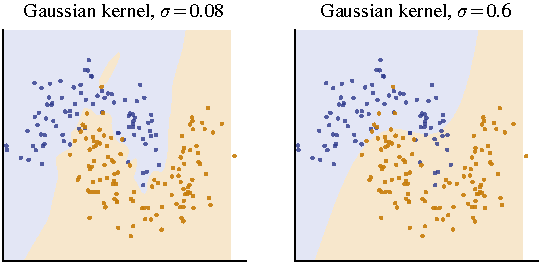
\includegraphics[width=0.72\linewidth]{figures/parzen_classifier.pdf}
\caption{Parzen-window classification of 200 points with a narrow and a wide Gaussian kernel.}
\label{fig:parzenclass}
\end{figure}

\paragraph{A numerical detail} For a query far from all data, or a small $\sigma$, every weight underflows to zero
and \eqref{eq:nw} becomes $0/0$. Since the ratio is unchanged when all weights are multiplied by a constant, subtract
the largest log-weight first:

\begin{verbatim}
def parzen_regress(Xtr, ytr, Xq, sigma):
    logW = -sq_distances(Xq, Xtr) / (2 * sigma**2)
    W = np.exp(logW - logW.max(axis=1, keepdims=True))   # largest weight is 1
    return (W @ ytr) / W.sum(axis=1)
\end{verbatim}

\begin{modern}{attention is kernel smoothing}
The attention operation at the heart of every transformer~\cite{vaswani2017} computes, for a query vector $\vect{q}$,
keys $\vect{k}_i$ and values $\vect{v}_i$,
\[
  \mathrm{Attention}(\vect{q}) = \sum_i \frac{\exp(\vect{q}\T\vect{k}_i / \sqrt{d})}{\sum_j \exp(\vect{q}\T\vect{k}_j / \sqrt{d})}\, \vect{v}_i ,
\]
which is \eqref{eq:nw} with an exponential kernel: each value votes with a weight set by the similarity of its key to
the query~\cite{tsai2019}. When queries and keys have unit norm, $\exp(\vect{q}\T\vect{k}/\tau)$ is a Gaussian kernel
in $\norm{\vect{q} - \vect{k}}$ (Exercise~E5). The ``subtract the maximum'' trick above is the same one used in every
implementation of softmax. What a transformer adds is that keys, queries and values are \emph{learned} functions of the
input, so the network learns which neighbours should vote.
\end{modern}

\section{Kernel density estimation}\label{sec:kde}

For density estimation there are no targets: each training point contributes a small bump of probability, and the
estimate is their average,
\[
  \hat p(\x) = \frac{1}{n}\sum_{i=1}^n K_h(\x - \x_i),
\]
where $K_h$ is itself a probability density of width $h$, typically the isotropic Gaussian $\Normal(\x; \x_i, h^2 I)$ of
Note~2. Because each bump is non-negative and integrates to one, so does $\hat p$. Unlike a histogram, the estimate
is smooth and does not depend on where bin edges happen to fall. The density panel of Note~1, Figure~1, was drawn this
way.

\begin{figure}[h]
\centering
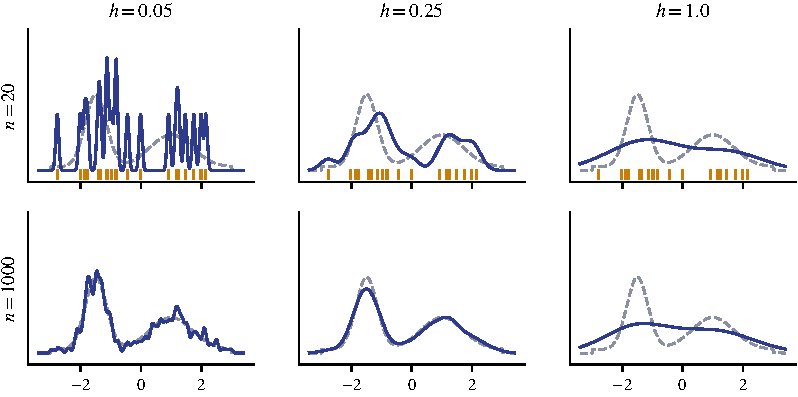
\includegraphics[width=\linewidth]{figures/kde.pdf}
\caption{Kernel density estimates (solid) of a two-peaked density with a uniform background (dashed), from $n = 20$
points (top; ticks mark the data) and $n = 1000$ points (bottom), for three bandwidths.}
\label{fig:kde}
\end{figure}

The bandwidth $h$ trades bias for variance (Figure~\ref{fig:kde}). A narrow kernel puts a spike on each data point;
a wide kernel blurs the two peaks into one. More data allow a narrower kernel. For a Gaussian kernel in one dimension
the normal-reference rule $h = 1.06\,\hat\sigma\, n^{-1/5}$ is a common starting point~\cite{silverman1986}; a more
reliable choice maximises the log-likelihood of held-out data, or the leave-one-out log-likelihood (Note~4). With the
best $h$ the mean squared error falls as $n^{-4/5}$ in one dimension --- faster than the $n^{-2/3}$ of histograms ---
but only as $n^{-4/(d+4)}$ in $d$ dimensions: kernels soften the curse of dimensionality without lifting it.

\begin{physics}{unbinned shapes}
When a particle-physics analysis needs the distribution of an observable for signal or background, but has only a
finite set of simulated events, kernel estimation provides a smooth, unbinned template; adaptive kernels whose width
grows in the tails, where events are scarce, are standard in the field~\cite{cranmer2001}.
\end{physics}

\section{Distances}\label{sec:distances}

Every method in this note is only as good as its notion of ``near''. A \emph{metric} on a set satisfies, for all
$\vect{a}, \vect{b}, \vect{c}$:
\begin{enumerate}
\item non-negativity: $d(\vect{a}, \vect{b}) \ge 0$, with $d(\vect{a}, \vect{b}) = 0$ if and only if $\vect{a} = \vect{b}$;
\item symmetry: $d(\vect{a}, \vect{b}) = d(\vect{b}, \vect{a})$;
\item triangle inequality: $d(\vect{a}, \vect{c}) \le d(\vect{a}, \vect{b}) + d(\vect{b}, \vect{c})$.
\end{enumerate}

\begin{minipage}[c]{0.6\linewidth}
\paragraph{Minkowski distances} $d_p(\vect{a}, \vect{b}) = \big(\sum_j |a_j - b_j|^p\big)^{1/p}$ for $p \ge 1$. The
cases $p = 1$ (Manhattan), $p = 2$ (Euclidean) and $p \to \infty$ ($\max_j |a_j - b_j|$) are the common ones. Their
unit balls (Figure~\ref{fig:balls}) show what each considers ``equally far''. For $p < 1$ the formula still measures
dissimilarity, but the triangle inequality fails (Exercise~E4).
\end{minipage}\hfill
\begin{minipage}[c]{0.36\linewidth}
\centering
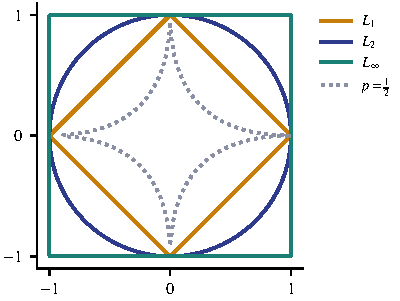
\includegraphics[width=\linewidth]{figures/unit_balls.pdf}
\captionof{figure}{Unit balls $\{\vect{a} : d_p(\vect{a}, \vect{0}) = 1\}$ in $\R^2$.}
\label{fig:balls}
\end{minipage}

\paragraph{Similarities for other data} For embeddings, the \emph{cosine similarity} $\vect{a}\T\vect{b} /
(\norm{\vect{a}}\norm{\vect{b}})$ ignores length and compares direction; for binary fingerprints, such as the
substructure bit vectors used to search chemical databases, the Tanimoto (Jaccard) similarity
$|\vect{a} \wedge \vect{b}| / |\vect{a} \vee \vect{b}|$ counts shared bits relative to bits set in either vector.

\paragraph{When Euclidean distance misleads} Three problems are common, each with a standard remedy.
\begin{itemize}
\item \emph{Units and scales.} A feature measured in GeV and another in radians contribute to the distance in
proportions set by the units. Standardise each feature with the mean and standard deviation of the training set
(Note~1, Section~5).
\item \emph{Correlations and irrelevant features.} Correlated features count the same information twice, and
irrelevant ones add noise to every distance. The Mahalanobis distance of Note~2 corrects for correlations; feature
selection or a learned projection removes irrelevant directions.
\item \emph{Invariances.} Two images of the same digit, shifted by two pixels, can be farther apart in pixel space
than images of different digits. \emph{Tangent distance} handles this by minimising the distance over small
transformations of one of the images~\cite{simard1993}.
\end{itemize}

\begin{modern}{learning the metric}
Today the distance is usually learned. Contrastive methods train a network so that two transformed views of the same
image map to nearby embeddings and views of different images map far apart~\cite{chen2020}; image--text models do the
same for an image and its caption~\cite{radford2021}. The invariances that tangent distance builds in by hand are
learned from the transformations used in training, and the plain cosine or Euclidean distance in the learned space
then works well for $k$-NN, retrieval and clustering.
\end{modern}

\begin{physics}{a metric for collider events}
Komiske, Metodiev and Thaler defined the distance between two collider events as the minimal ``work'' needed to
rearrange one event's energy flow into the other's --- an optimal-transport, or earth mover's, distance --- which
respects the physical requirement that soft or collinear emissions should change it only slightly~\cite{komiske2019}.
With this metric, a $k$-NN classifier on jets performs competitively, and geometric quantities of the space of events
become measurable. Choosing the distance is where the physics enters.
\end{physics}

\begin{keyidea}[Summary]
$k$-NN and Parzen windows predict by a weighted vote of training examples, with weights given by neighbourhood
membership or by a kernel; the same formula serves regression, classification and, without targets, density
estimation. They need no training, are consistent as $n \to \infty$, and have one main hyperparameter --- $k$ or the
width --- that trades bias for variance. Prediction costs $O(nd)$ per query unless approximate search is used. Their
weak point is the distance: it must reflect the problem's units, correlations and invariances, which is why modern
systems learn the representation and then use simple neighbourhood methods on top of it.
\end{keyidea}

\begin{exercises}
\item Show that the 1-NN decision boundary between two training points of different classes lies on their
perpendicular bisector. Sketch the Voronoi cells and the boundary for the four points $(0,0)$, $(2,0)$, $(0,2)$,
$(2,2)$ labelled $+, -, -, +$.
\item Implement \texttt{knn\_classify} and generate data of your own with two interleaved classes. Choose $k$ by
5-fold cross-validation and plot the validation error against $k$. How does the selected $k$ change when you double
$n$?
\item Show that the kernel density estimate integrates to one, and that $\E[\hat p(\x)] = \int K_h(\x - \vect{u})\,
p(\vect{u})\, d\vect{u}$. Conclude that for fixed $h$ the estimate stays biased however large $n$ is, and explain why
$h$ must decrease with $n$, but not too fast.
\item Find three points in $\R^2$ for which $d_{1/2}$ violates the triangle inequality.
\item Let $\norm{\vect{q}} = \norm{\vect{k}_i} = 1$. Show that $\exp(\vect{q}\T\vect{k}_i / \tau)$ is proportional
to a Gaussian kernel in $\norm{\vect{q} - \vect{k}_i}$ and find its width. What happens to attention as
$\tau \to 0$?
\item A retrieval system stores $10^7$ embeddings in $\R^{768}$ as 32-bit floats. How much memory do they take, and
how many multiply--add operations does one brute-force query need? At $10^{12}$ operations per second, how many queries
per second is that?
\end{exercises}

\paragraph{Further reading} Hastie, Tibshirani and Friedman~\cite{hastie2009}, sections~2.3, 6.1--6.6 and 13.3;
Silverman~\cite{silverman1986} for kernel density estimation.

\begin{thebibliography}{99}\small
\bibitem{chen2020} T.~Chen, S.~Kornblith, M.~Norouzi and G.~Hinton, A simple framework for contrastive learning of visual representations, \emph{ICML} (2020).
\bibitem{cover1967} T.~M. Cover and P.~E. Hart, Nearest neighbor pattern classification, \emph{IEEE Trans.\ Inf.\ Theory} 13, 21--27 (1967).
\bibitem{cranmer2001} K.~Cranmer, Kernel estimation in high-energy physics, \emph{Comput.\ Phys.\ Commun.}\ 136, 198--207 (2001).
\bibitem{hastie2009} T.~Hastie, R.~Tibshirani and J.~Friedman, \emph{The Elements of Statistical Learning}, 2nd ed., Springer (2009).
\bibitem{johnson2021} J.~Johnson, M.~Douze and H.~Jégou, Billion-scale similarity search with GPUs, \emph{IEEE Trans.\ Big Data} 7, 535--547 (2021).
\bibitem{khandelwal2020} U.~Khandelwal \emph{et al.}, Generalization through memorization: nearest neighbor language models, \emph{ICLR} (2020).
\bibitem{komiske2019} P.~T. Komiske, E.~M. Metodiev and J.~Thaler, Metric space of collider events, \emph{Phys.\ Rev.\ Lett.}\ 123, 041801 (2019).
\bibitem{lewis2020} P.~Lewis \emph{et al.}, Retrieval-augmented generation for knowledge-intensive NLP tasks, \emph{NeurIPS} (2020).
\bibitem{malkov2020} Y.~A. Malkov and D.~A. Yashunin, Efficient and robust approximate nearest neighbor search using hierarchical navigable small world graphs, \emph{IEEE Trans.\ Pattern Anal.\ Mach.\ Intell.}\ 42, 824--836 (2020).
\bibitem{radford2021} A.~Radford \emph{et al.}, Learning transferable visual models from natural language supervision, \emph{ICML} (2021).
\bibitem{silverman1986} B.~W. Silverman, \emph{Density Estimation for Statistics and Data Analysis}, Chapman \& Hall (1986).
\bibitem{simard1993} P.~Simard, Y.~LeCun and J.~S. Denker, Efficient pattern recognition using a new transformation distance, \emph{NeurIPS} (1993).
\bibitem{stone1977} C.~J. Stone, Consistent nonparametric regression, \emph{Ann.\ Statist.}\ 5, 595--620 (1977).
\bibitem{tsai2019} Y.-H.~H. Tsai \emph{et al.}, Transformer dissection: a unified understanding of transformer's attention via the lens of kernel, \emph{EMNLP} (2019).
\bibitem{vaswani2017} A.~Vaswani \emph{et al.}, Attention is all you need, \emph{NeurIPS} (2017).
\end{thebibliography}

\SourceNote
\end{document}
